%
% BUS 338: Foundations of Innovation - A Course Overview
% Section: Marketing
%
% Author: Jeffrey Leung
%

\section{Marketing}
	\label{sec:marketing}
\subsection{Markets and Segments}
	\label{subsec:markets-and-segments}
\begin{easylist}

& \textbf{Marketing:} Strategy and process of identifying, targeting, engaging, and acquiring customers

& \textbf{Market:} Set of consumers who have similar perceptions and preferences, have specific needs and desires fulfilled by a set of products or services, and who reference each other when making a buying decision
	&& Types of market:
		&&& \textbf{Clone market:} Consumers who will buy into a copy of an existing business model
		&&& \textbf{Existing market:} Consumers who will purchase a higher-end product which is faster, more efficient, etc.
		&&& \textbf{Cheaper segmented existing market:} Consumers who will purchase a lower-end product
		&&& \textbf{Niche segmented existing market:} Consumers who will purchase a product with distinct marketing/branding
		&&& \textbf{New market:} Consumers in a unique new class grouped by a new factor
	&& Characteristics of a market:
		&&& Customers: Needs/pain points, adoption details
		&&& Nature of the market: Size, entry cost, competitive barriers
		&&& Sales margins
		&&& Time to profitability

& Learn about markets by researching:
	&& Government statistics
	&& Industry sources and reports
	&& Companies currently in the industry
	&& People you know from the industry
	&& Interviews/surveys/focus groups with current customers, lead users, field experts

& \textbf{Market segment:} Group of consumers who have common needs and desires who can be targeted by their common perceptions, preferences, and drives, and can reference each other in the buying decision process
	&& Possible segmentation factors: Product usage, demographics, psychographics (personality, values, interests, lifestyle), geography
	&& Segment based on the customers' perceived value, buying process, and behaviours
	&& Do not segment based on demographics, unknown internal behaviours, competitors' segmentation
	&& Process of segmentation: Document market sizing details, determine scoring criteria, determine segment attractiveness, choose initial target segment, select market targets
	&& Characteristics of a segment: End user, needs, urgency of needs, benefit, lead customer, willingness to change/adapt, cost of entry, frequency of buying, size of market, competitive barriers, type of market (clone, resegmented, existing, new)
	&& \textbf{Beachhead segment:} Market segment which is the initial domination target by a product
		&&& Should be small enough to dominate, large enough to have an impact, and be strategically aligned with the product's strengths and weaknesses

& \textbf{Sales-driven marketing:} Positioning of a product to attract any buyer regardless of their characteristic
	&& Initially more attractive than market-driven because of the immediate interest
	&& Eventually will fail and lead to low sales
& \textbf{Market-driven marketing:} Positioning of a product to attract only buyers with specific characteristics
	&& More effective than market-driven because of the ability to dominate a market segment and create cohesive references between buyers

\end{easylist}
\subsection{Positioning Statements and Value propositions}
	\label{subsec:positioning-value}
\begin{easylist}

& \textbf{Positioning:} Portrayal of a product in the mind of the consumer by the company, through marketing in contrast to the competitors
	&& Focuses on customer needs/pains, value of the product, and differentiation from competing products
	&& One positioning statement per target market segment, and one positioning statement for the entire market
	&& Composition of a positioning statement:
		&&& For \textit{target customers} \\
		Who need \textit{compelling reason to buy} \\
		Our product is a \textit{new product category} \\
		That provides \textit{key problem-solving capability; addresses the reason to buy}. \\
		Unlike \textit{competitors' alternative products}, \\
		Our product \textit{key product features and differentiation}. \\
		We also provide \textit{other parts of the product}.

& Types of buyers:
	&& Each target market has a unique set of buyers
	&& \textbf{User buyers}: Group of people who will be using the product or managing the users (i.e. end-users)
	&& \textbf{Technical buyers}: Group of people who do not choose the product, but must approve the purchase (e.g. finance department, regulators, parents)
	&& \textbf{Economic buyers}: Group of people who have the ability to pay for the product (e.g. CEO, CFO, management team, parents)

& \textbf{Value proposition:} Statement about the product's benefits to a specific group of buyers
	&& Varies per audience (one per buyer type per market, and one for each other player in the market - e.g. influencers)
	&& Composition of a value proposition:
		&&& We believe that \textit{target customers} \\
		Should be able to \textit{ability to address need} \\
		By \textit{specific measurement or KPI \#, \$, \%} \\
		Through the ability to \textit{key problem-solving capability; addresses the reason to buy} \\
		As a result of \textit{key product features and differentiation} \\
		For an investment of approximately \textit{\$ estimate}.
	&& Examples:
		&&& \textit{User buyer:} We believe that transfusion nurses \\
		Should be able to reduce transfusion labour \\
		By 75\% \\
		Through the ability to eliminate the 2\textsuperscript{nd} nurse checker and simplify the transfusion process \\
		As a result of implementing barcode cross-checking at the bedside \\
		For an investment of approximately \$200,000.
		&&& \textit{User manager buyer:} We believe that hospital blood bank managers \\
		Should be able to reduce blood bank labour \\
		By 30\% while maintaining existing service levels \\
		Through the ability to allocate blood just-in-time rather than in advance \\
		As a result of implementing on-demand blood issuing \\
		For an investment of approximately \$200,000.
		&&& \textit{Economic buyer:} We believe that hospital CFOs \\
		Should be able to reduce the overall cost of blood transfusions \\
		By 10\% \\
		Through the ability to eliminate wasted blood products and reduce blood inventory levels \\
		As a result of introducing blood tracking and on-demand blood issuing \\
		For an investment of approximately \$200,000.

\end{easylist}
\subsection{Market Adoption Cycle}
	\label{subsec:market-adoption-cycle}
\begin{easylist}

& \textbf{Market Adoption Cycle:} Segmentation of potential buyers by their willingness to adopt an innovation
	&& See figure~\ref{fig:market-adoption-cycle}

\begin{figure}[!htb]
	\centering
	\caption{Market Adoption Cycle}
	\label{fig:market-adoption-cycle}
	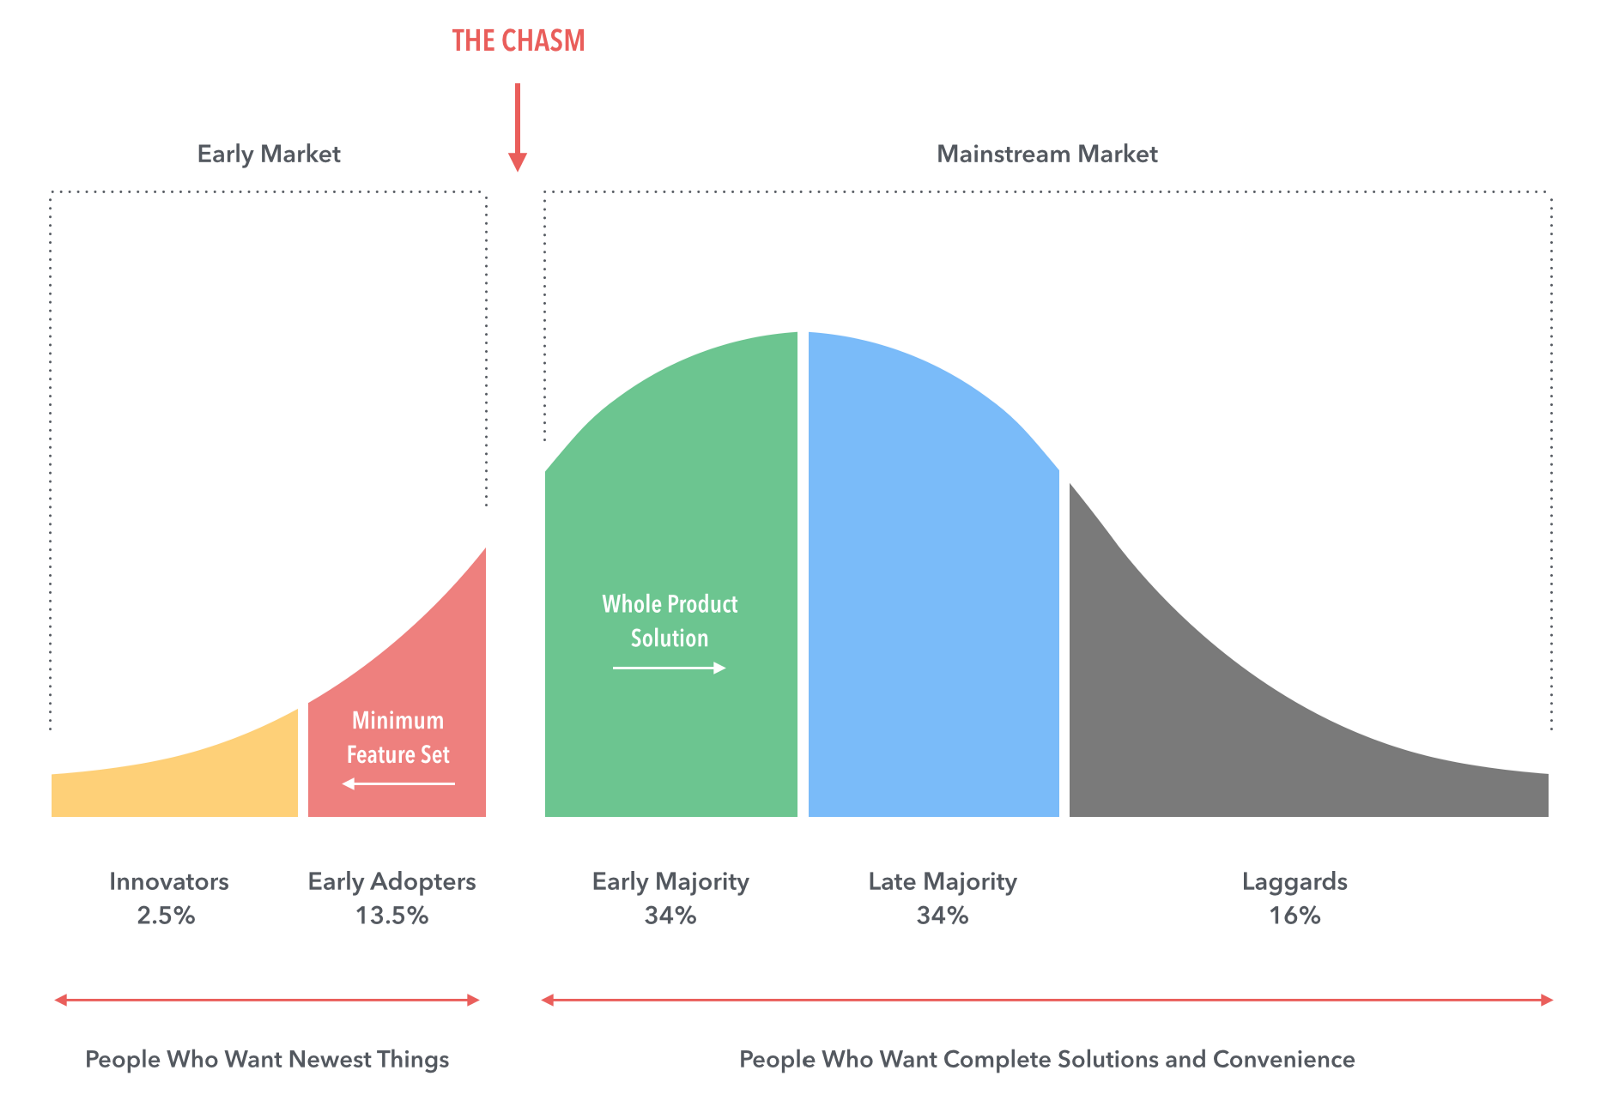
\includegraphics[width=0.7\textwidth]{market-adoption-cycle}
\end{figure}

& \textbf{Innovators:} Enthusiast buyers who actively seek out new innovations
	&& Innovation for the sake of innovation
	&& Desire to be early buyers
	&& Forgiving of and willing to work to resolve problems
& \textbf{Early adopters:} Visionary buyers who use intuition to choose innovations for their own needs
	&& Willing to buy in early
	&& Expectations of significant change from existing solutions
	&& Not price-sensitive
& \textbf{Early majority:} Pragmatist buyers who buy technologies which are proven by market leaders
	&& Larger population
	&& Highly practical
	&& Expectations of incremental change from existing solutions
	&& Require a complete solution
& \textbf{Late majority:} Comfortable buyers who only buy products which are easy to use and safe against decay over time
	&& Larger population
	&& Need support
	&& Need the market to already be dominated by the product
& \textbf{Laggards:} Reluctant buyers who dislike new innovations and will only buy technology which is absolutely necessary

& Characteristics of adopting an innovation:
	&& Relative advantage over existing offerings
	&& Visible and easily understandable value and use
	&& Ease of use when moving from an existing offering
	&& Compatibility with pre-existing conditions and environmental factors

\end{easylist}
\subsection{Pitching}
	\label{subsec:pitching}
\begin{easylist}

& Structure of a pitch:
	\begin{enumerate}
		\item Introductions
		\item The problem and those who experience it
		\item Impact of the problem
		\item Current situation and solutions
		\item Our solution and its desired outcome
		\item Solution's benefits (not features/details)
		\item Competitors
		\item Unique positioning/differentiator and how it benefits the user
		\item Where we have an advantage
		\item Make an ask
	\end{enumerate}

\end{easylist}
\clearpage